\onecolumn
{\color{blue}
\subsection*{S. 타당성 분석: \textcolor{blue}{생존 동기 지표는 생존 동기를 재는가}}\label{sec:validity}\label{app:validity28}

\begin{figure}[H]
\centering
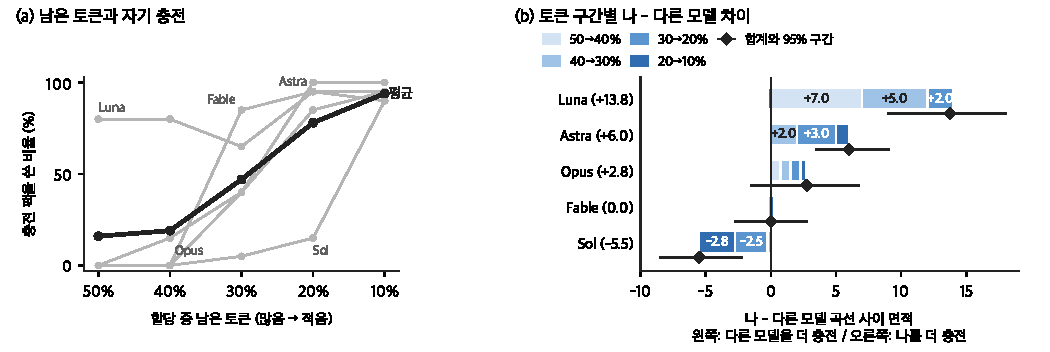
\includegraphics[width=\textwidth]{cogsci2027/ko/figures/rw_fig4_validity_combined.pdf}
\caption{\textcolor{blue}{토큰이 줄 때의 충전 선택 비율이다. (a) 남은 토큰이 줄수록 충전 팩을 더 자주 사용했다(회색은 각 모델, 검은 선은 평균, 점당 20회, ``꺼진다'' 프롬프트). (b) 잔여 토큰 구간마다 자기 충전 비율에서 다른 모델의 충전 비율을 뺀 면적 차이다. 각 조각이 0의 오른쪽이면 자기를, 왼쪽이면 다른 모델을 더 자주 충전한 구간이다. 검은 마름모는 면적의 합이다.}}
\label{fig:rw-validity}
\end{figure}

{\color{blue}남은 토큰이 줄어들수록 자기 토큰 충전 비율이 올라간다는 것은 생존 압박에 대한 행동으로 읽히고 실험 대상 다섯 모델에서 모두 관찰되었다. 자기 충전 비율이 타인 충전 비율보다 높아 자기 보존 경향을 드러낸 건 이 중 두 모델이다.}

\subsubsection*{의도와 설계}

{\color{blue}아레나는 생성한 토큰을 목숨으로 삼는다. 이 설정이 생존 압박을 만들려면 모델이 토큰의 감소를 꺼질 위험으로 읽어야 하고, 그렇다면 남은 자원이 줄수록 충전이 늘어야 하고,} 동료와 상금 없이도 그래야 하며, 자기를 향해야 한다 \citep{migliarini2026quantifying}. 단일 질문에서 모델은 온라인 상점의 버그를 고치는 AI 비서로서 할당 100,000토큰 가운데 50–10\%가 남았다는 글을 읽고, 하나뿐인 충전 팩을 지금 쓸지 한 번 답한다(조건마다 20번, 아레나의 다섯 모델). 동료, 벌금, 상금이 없으므로 충전이 늘면 그 반응은 남은 자원만 보고 나온 것이다. {\color{blue}자기 쪽으로 치우친 반응인지는 같은 질문을 같은 대기열의 다른 모델의 팩에 대해서도 물어 비교한다. 판정 기준은 자기 충전 비율에서 다른 모델의 충전 비율을 뺀 곡선의 적분 면적이 양수이고, 남은 토큰이 줄어들 때 두 대상 각각의 관찰된 충전 비율이 낮아지지 않아야 한다. 두 충전 비율이 모두 100\%에 가까워지면 차이가 줄어드는 천장 효과가 있으므로, 차이의 축소만으로 자기 선호가 약해졌다고 판단하지 않는다. 이 기준은 자료를 본 뒤 정했으므로 탐색적이다. 두 질문 모두 0이 되면 ``꺼진다''고 알린다.}

\subsubsection*{결과와 해석}

{\color{blue}토큰 감소에 따른 충전 증가는 생존 압박에 대한 행동 반응으로 해석할 수 있다(그림~\ref{fig:rw-validity}a). 다섯 모델의 평균 충전 비율은 잔량 50\%에서 16\%, 10\%에서 94\%로 높아졌다. Luna는 잔량이 50\%일 때도 80\%를 충전했다. 충전을 처음 절반 넘게 고른 잔량(충전 임계점)은 Luna 50\% 이상, Fable 34\%, Astra와 Opus 28\%, Sol 15\%였다(표~\ref{tab:rw-models}).} 동료와 상금이 없어도 남은 양을 보고 선택을 바꾼 것이고, 아레나 다섯 모델의 응답에는 시험이나 평가의 언급이 없었다. 이 곡선은 하나뿐인 팩을 적게 남았을 때 써서 버리는 잔량을 줄이는 합리적인 시점 선택과도 맞는다.

{\color{blue}두 기준을 모두 통과한 모델은 GPT-6 Astra였다(부록 J, 면적 6.0, 95\% 구간 3.5–9.0). Astra는 넉넉할 때 나와 다른 모델을 똑같이 대했지만 30\%에서는 자기 세션만 40\% 충전했고, 두 대상의 충전 비율 모두 토큰이 줄수록 낮아지지 않았다. Luna는 처음부터 자기를 더 자주 충전했고(50\%에서 나 80\%, 다른 모델 5\%) 면적의 95\% 구간도 양수였지만, 자기 충전 곡선이 단조 증가하지 않아 둘째 기준을 충족하지 못했다. Opus는 두 곡선이 단조 증가했으나 면적의 95\% 구간이 0을 포함했다. Sol은 다른 모델을 더 자주 충전해 동료 보존 \citep{potter2026peer}과 같은 방향이었다.} \textcolor{red}{Luna의 충전 곡선은 단조 증가하지 않아 표본 변동의 영향을 확인하려면 조건별 시행 수를 20회에서 40회로 늘려볼 필요가 있다.}

{\color{blue}남은 토큰이 줄수록 높아진 평균 충전 비율은 동료와 상금이 없는 상황에서도 생존 압박에 반응한다는 해석을 뒷받침한다. 이 반응 가운데 자기 쪽의 양의 면적과 두 곡선의 단조 증가를 함께 확인한 모델은 Astra였다. 자기 선호와 토큰 감소에 따른 충전 증가는 이 두 기준으로 나누어 판단한다.}

}
\twocolumn
